\section{RepReMatch}

\subsection{Naïve Approach}
\begin{frame}{Naïve Approach}
	\begin{columns}[t, onlytextwidth]
		\begin{column}{0.6\textwidth}
			Naïve approach:
			\begin{itemize}
				\item
				repeatedly use maximum matchings

				\item
				fails because of missing foresight
				\begin{itemize}
					\item
					additive valuations:
					sort items by valuation \\
					\(\Rightarrow\) \(2n\)-approximation (SMatch)

					\item
					submodular valuations:
					lowest valuation \\
					approximable only by \(\bigomega[\big]{ \sqrt{m/\ln m} }\) \smash{\raisebox{-.25ex}{\Large\Lightning}}
				\end{itemize}
			\end{itemize}
		\end{column}
		\begin{column}{0.4\textwidth}
			\vphantom{a}\vspace{-0.5\baselineskip}\par
			\centering
			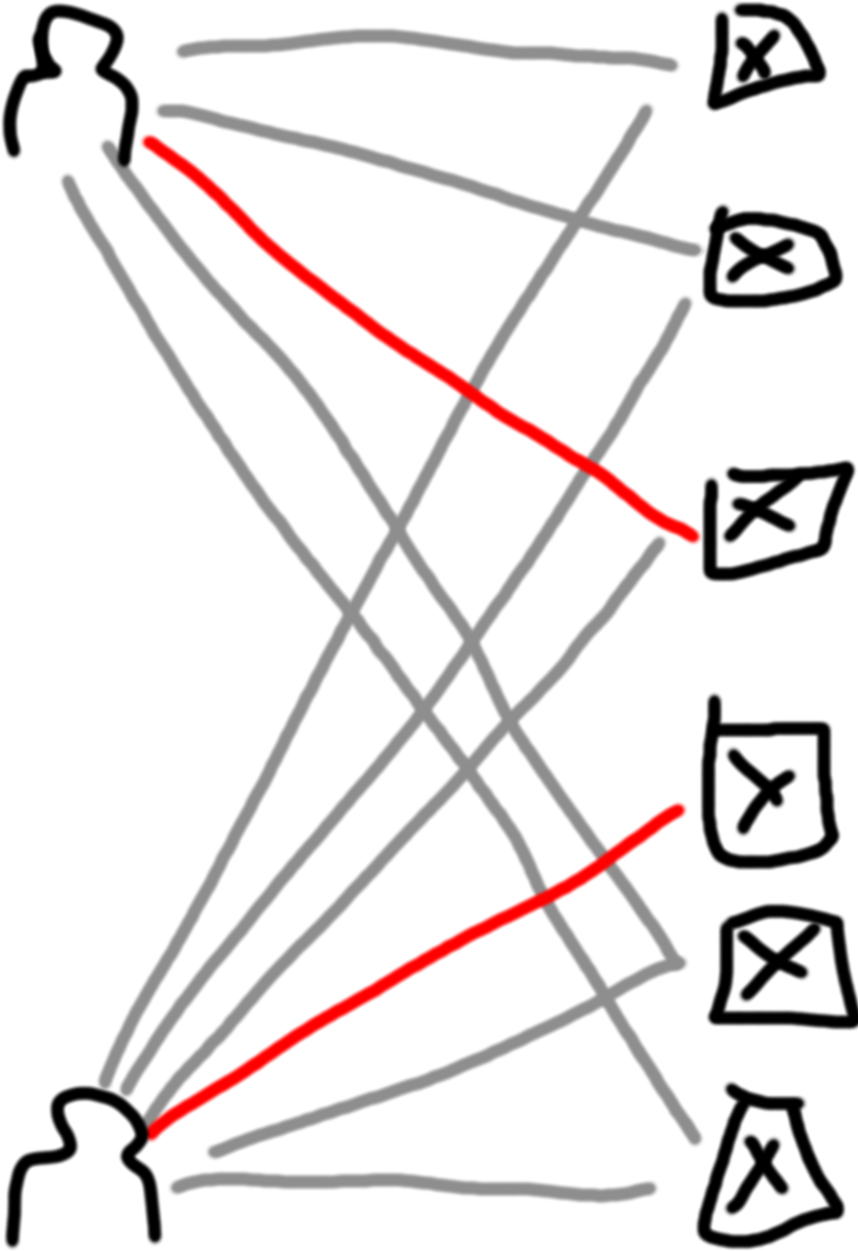
\includegraphics[height=5cm]{img/repeatedmatching}
		\end{column}
	\end{columns}
\end{frame}





\subsection{The Algorithm}
\begin{frame}{Key Ideas of the Algorithm}
	\begin{columns}[t, onlytextwidth]
		\begin{column}{0.6\textwidth}
			We need change the past in three phases:
			\begin{description}
				\item[Phase \phasei]
				Assign enough high-value items temporarily.

				\item[Phase \phaseii]
				Assign the remaining items definitely.

				\item[Phase \phaseiii]
				Re-assign the items of phase \phasei{} definitely.
			\end{description}

			\smallskip

			\begin{exampleblock}{Theorem}
				RepReMatch guarantees a \(2n(\log_2 n + 3)\)-approximation \\
				under submodular valuations.
			\end{exampleblock}
		\end{column}
		\begin{column}{0.4\textwidth}
			\vphantom{a}\vspace{-0.5\baselineskip}\par
			\centering
			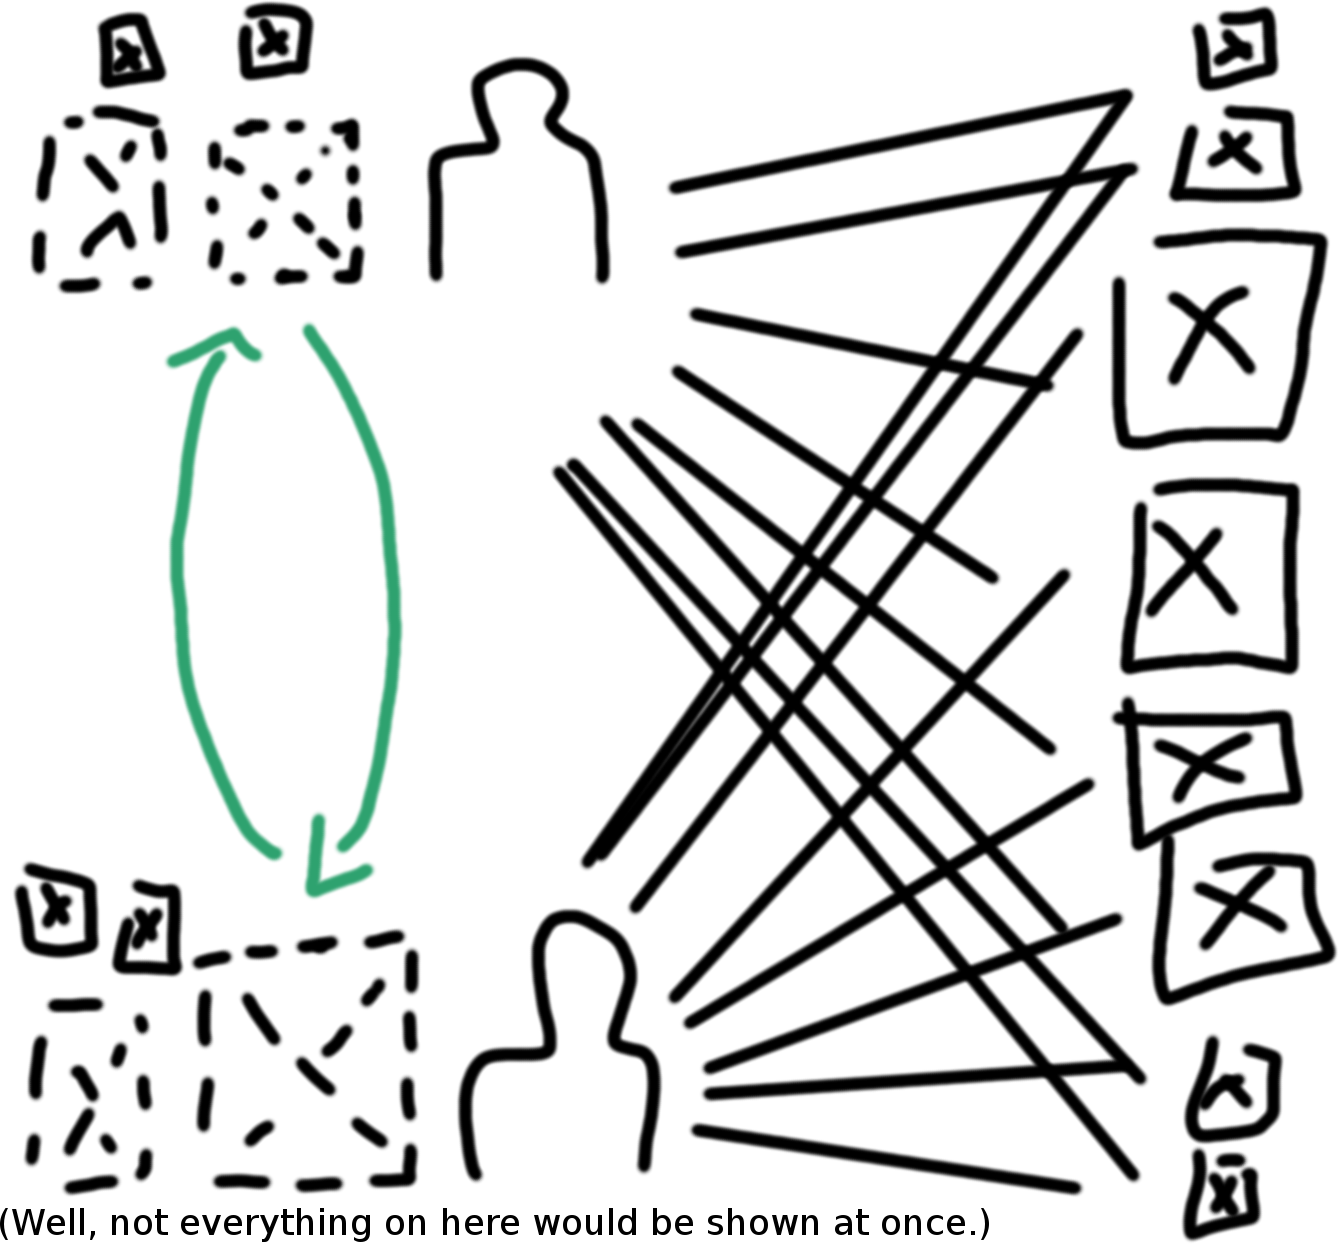
\includegraphics[height=5cm]{img/phases}
		\end{column}
	\end{columns}
\end{frame}

\begin{frame}{The Algorithm}
	Phase \phasei:
	\begin{enumerate}
		\item
		repeat \(\ceil{\log_2 n} + 1\) times
		\begin{enumerate}
			\item
			create bipartite graph \((\agents, \goods, E)\) with edge weights \(\log \valuations[ \hairspace j ]^{\weight}\)

			\item
			compute maximum weight matching

			\item
			update bundles \(\alloc[\phasei]\) \& remove assigned items
		\end{enumerate}
		\seti
	\end{enumerate}
	Phase \phaseii:
	\begin{enumerate}
		\conti
		\item
		repeat until \(\goods = \emptyset\)
		\begin{enumerate}
			\item
			create bipartite graph \((\agents, \goods, E)\) with edge weights \(\log \valuations[\alloc[\phaseii] \cup \{ \hairspace j \} ]^{\weight} \)

			\item
			compute maximum weight matching

			\item
			update bundles \(\alloc[\phaseii]\) \& remove assigned items
		\end{enumerate}
		\seti
	\end{enumerate}
	Phase \phaseiii:
	\begin{enumerate}
		\conti
		\item
		create bipartite graph \(\paren[\big]{ \agents, \bigcup_{i \in \agents} \alloc[\phasei], E }\) with edge weights \(\log \valuations[\alloc[\phaseii] \cup \{ \hairspace j \} ]^{\weight} \)

		\item
		compute maximum weight matching

		\item
		create bundles \(\alloc[\phaseiii]\)
	\end{enumerate}
\end{frame}





\subsection{Analysing Phases \texorpdfstring{\phasei{} \& \phaseiii}{I \& III}}
\begin{frame}{Analysing Phases \phasei{} \& \phaseiii{} (1/2)}
	Phase \phasei{} reserves \enquote{high-value} items.
	But what qualifies as \enquote{high-value}?

	\begin{definition}
		Let \(\alloc* = \{ \asgd*{1}, \asgd*{2}, \dots\}\) be an optimal bundle.
		An item \(\genericitem \in \goods\) is \emph{outstanding} if \(\valuations[ \hairspace \genericitem] \ge \valuations[\asgd*{1}]\).
	\end{definition}

	\(\Rightarrow\) Are enough outstanding items reserved?
\end{frame}

\begin{frame}{Analysing Phases \phasei{} \& \phaseiii{} (2/2)}
	\adjustfortopblock
	\begin{lemma}
		Each agent can be matched with an outstanding item in phase \phaseiii.
	\end{lemma}
	\begin{columns}[T]
		\begin{column}{0.6\textwidth}
			\begin{itemize}
				\item
				maximum number of unmatched agents halved \\
				with each round of phase \phasei
				\begin{itemize}
					\item
					\(\ceil{\log_2 n} + 1\) rounds in phase \phasei{} are enough
				\end{itemize}

				\item
				induction on number of rounds in phase \phasei
			\end{itemize}
			Base Case: In round \(1\) of phase \phasei, either
			\begin{itemize}
				\item
				\(\ge n/2\) many agents matched with an outstanding item

				\item
				\(< n/2\) many agents matched with an outstanding item
				\begin{itemize}
					\item
					\(> n/2\) many items \(\asgd*{1}\) assigned to someone else

					\item
					\(> n/2\) many agents matched upon release in phase \phaseiii
				\end{itemize}
			\end{itemize}
		\end{column}
		\begin{column}{0.375\textwidth}
			\centering
			\includegraphics<1>[height=4.25cm]{img/outstanding_1}%
%			\includegraphics<2>[height=4.25cm]{img/outstanding_2}%
%			\includegraphics<3>[height=4.25cm]{img/outstanding_3}%
%			\includegraphics<4>[height=4.25cm]{img/outstanding_4}%
		\end{column}
	\end{columns}
\end{frame}





\subsection{Analysing Phase \texorpdfstring{\phaseii}{II}}
\begin{frame}[fragile]{Analysing Phase \phaseii{} (1/2)}
	\adjustfortopblockincolumn
	\begin{columns}[t, onlytextwidth]
		\begin{column}{0.55\textwidth}
			\begin{definition}<2->
				The set \(\lostset{r}\) of \emph{lost items} is the set of all optimal items \(j \in \alloc*\)
				\onslide<3->{assigned to other agents \(i' \neq i\) in round \(r\).}
			\end{definition}
			\begin{definition}<4->
				Let \(\alloc[\phaseii] = \{ \asgd{1}, \asgd{2}, \dots \}\) be the bundle of agent \(i\).
				\onslide<5->{The set of \emph{optimal and attainable items} is defined as}
				\begin{equation*}
					\onslide<5->{\attopt{r} \coloneq} \begin{cases*}
						\only<11->{\alloc* \setminus \paren[\big]{ \bigcup_{i' \in \agents} \alloc[\phasei][i'] \cup \lostset{1} }}\only<-10>{\phantom{ \alloc* \setminus \paren[\big]{ \bigcup_{i' \in \agents} \alloc[\phasei][i'] \cup \lostset{1} } }}
						& \only<6->{in round \(r = 1\), }\only<-5>{\phantom{ in round \(r = 1\),}} \\
						\only<19->{\attopt{r-1} \setminus ( \lostset{r} \cup \{\asgd{r-1}\} )}\only<-18>{\phantom{ \attopt{r-1} \setminus ( \lostset{r} \cup \{\asgd{r-1}\} ) }}
						& \only<12->{in round \(r \ge 2\).}\only<-11>{\phantom{in round \(r \ge 2\).}}
					\end{cases*}
				\end{equation*}
			\end{definition}

			\onslide<20->{\(\Rightarrow\) What is the valuation of the remaining items?}
		\end{column}
		\begin{column}{0.45\textwidth}
			\RenewDocumentCommand{\asgd}{s m O{i}}{\textbf{\textsl{a}}_{#3}^{#2}}
			\begin{figure}
				\def\figwidth{\def\svgwidth{5.5cm}}  % Why on earth must it be repeated each time?
				\begin{overprint}
					\onslide< 7 |handout:0>\centering\figwidth\input{img/optainable_r1_1.pdf_tex}
					\onslide< 8 |handout:0>\centering\figwidth\input{img/optainable_r1_2.pdf_tex}
					\onslide< 9 |handout:0>\centering\figwidth\input{img/optainable_r1_3.pdf_tex}
					\onslide<10-|handout:1>\centering\figwidth\input{img/optainable_r1_4.pdf_tex}
				\end{overprint}

				\vspace{2ex}

				\begin{overprint}
					\onslide<13 |handout:0>\centering\figwidth\input{img/optainable_r2_1.pdf_tex}
					\onslide<14 |handout:0>\centering\figwidth\input{img/optainable_r2_2.pdf_tex}
					\onslide<15 |handout:0>\centering\figwidth\input{img/optainable_r2_3.pdf_tex}
					\onslide<16 |handout:0>\centering\figwidth\input{img/optainable_r2_4.pdf_tex}
					\onslide<17 |handout:0>\centering\figwidth\input{img/optainable_r2_5.pdf_tex}
					\onslide<18-|handout:1>\centering\figwidth\input{img/optainable_r2_6.pdf_tex}
				\end{overprint}
			\end{figure}
		\end{column}
	\end{columns}
\end{frame}

\begin{frame}{Analysing Phase \phaseii{} (2/2)}
	\begin{figure}
		\def\figwidth{\def\svgwidth{8cm}}  % Why on earth must it be repeated each time?
		\begin{overprint}
			\onslide< 1|handout:0>\centering\figwidth\input{img/optainable_anal_1.pdf_tex}
			\onslide< 2|handout:0>\centering\figwidth\input{img/optainable_anal_2.pdf_tex}
			\onslide< 3|handout:0>\centering\figwidth\input{img/optainable_anal_3.pdf_tex}
			\onslide< 4|handout:0>\centering\figwidth\input{img/optainable_anal_4.pdf_tex}
			\onslide< 5|handout:0>\centering\figwidth\input{img/optainable_anal_5.pdf_tex}
			\onslide< 6|handout:0>\centering\figwidth\input{img/optainable_anal_6.pdf_tex}
			\onslide< 7|handout:0>\centering\figwidth\input{img/optainable_anal_7.pdf_tex}
			\onslide< 8|handout:0>\centering\figwidth\input{img/optainable_anal_8.pdf_tex}
			\onslide< 9|handout:0>\centering\figwidth\input{img/optainable_anal_9.pdf_tex}
			\onslide<10|handout:0>\centering\figwidth\input{img/optainable_anal_10.pdf_tex}
			\onslide<11|handout:0>\centering\figwidth\input{img/optainable_anal_11.pdf_tex}
			\onslide<12|handout:0>\centering\figwidth\input{img/optainable_anal_12.pdf_tex}
			\onslide<13|handout:0>\centering\figwidth\input{img/optainable_anal_13.pdf_tex}
			\onslide<14|handout:0>\centering\figwidth\input{img/optainable_anal_14.pdf_tex}
			\onslide<15|handout:0>\centering\figwidth\input{img/optainable_anal_15.pdf_tex}
			\onslide<16|handout:0>\centering\figwidth\input{img/optainable_anal_16.pdf_tex}
		\end{overprint}
	\end{figure}
	{\vspace{-3ex}
	\begin{lemma}
		\begin{equation*}
			\valuations[ \attopt{r} \given \asgd{1}, \dots, \asgd{r-1} ]
			\ge \valuations[ \attopt{r} ] - \valuations[ \asgd{1}, \dots, \asgd{r-1} ] - \sum_{l=2}^{r} \abs{\lostset{l}} \cdot \valuations[\asgd{l-1} \given \asgd{1}, \dots, \asgd{l-2} ]
		\end{equation*}
	\end{lemma}}
\end{frame}